% Dokumentinformationen
\title{ElMasch - Zusammenfassung}
\author{Gregor Dengler}
\documentclass[10pt,twoside,a4paper,fleqn]{article}

% Header
\usepackage{paralist}
\include{header/zusammenfassung}


% Document
\begin{document}
\setcounter{tocdepth}{2} 	%Es wird nur bis Subsection im Inhaltsverzeinichs angezeigt
\tableofcontents 				%Inhaltsverzeichnis
\newpage
\section{Die elektrodynamischen Grundgesetze}
\subsection{Elektrische Kraft und elektrisches Feld}

\begin{minipage}{0.4 \linewidth}
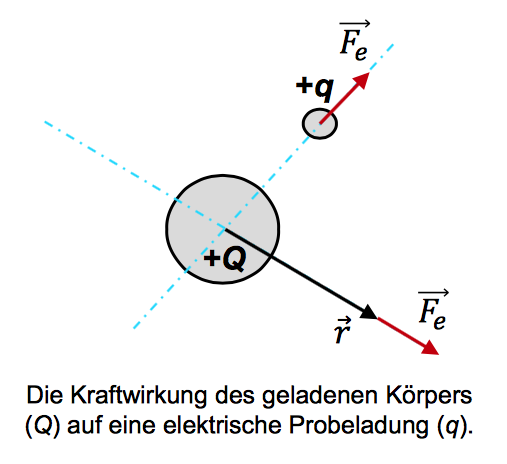
\includegraphics[width = \linewidth]{./Pics/VL1/elKraft}
\end{minipage}
\begin{minipage}{0.5 \linewidth}
Die elektrische Kraft zwischen unendlichen parallelen Leitern:

$\vec{F_{e}} = \frac{1}{2 \pi \epsilon} \cdot \frac{Qq}{r} \cdot \vec{r_{0}} (\frac{N}{m})$ \\

$\epsilon$ - dielektrische Permittivität \\
$\epsilon_{0}$ - die Permittivität des Vakuums \\
$\epsilon_{0} = 8.85 \cdot 10^{-12}$ $(\frac{As}{Vm})$ \\
$Q,q$ - Linienladungsdichten $(\frac{C}{m})$ \\
$\vec{r_{0}} = \frac{\vec{r}}{|\vec{r}|} $ - Einheitsvektor\\
\end{minipage}

\begin{minipage}{0.5 \linewidth}
Das elektrische Feld wird als die elektrische Kraft auf die Einheitsladung definiert:
\begin{equation}
\vec{E} = \frac{\vec{F_{e}}}{q} \ (\frac{V}{m})
\vec{E} = \frac{1}{2 \pi \epsilon} \cdot \frac{Q}{r} \cdot \vec{r_{0}}(\frac{V}{m})
\end{equation}
\end{minipage}
\begin{minipage}{0.4 \linewidth}
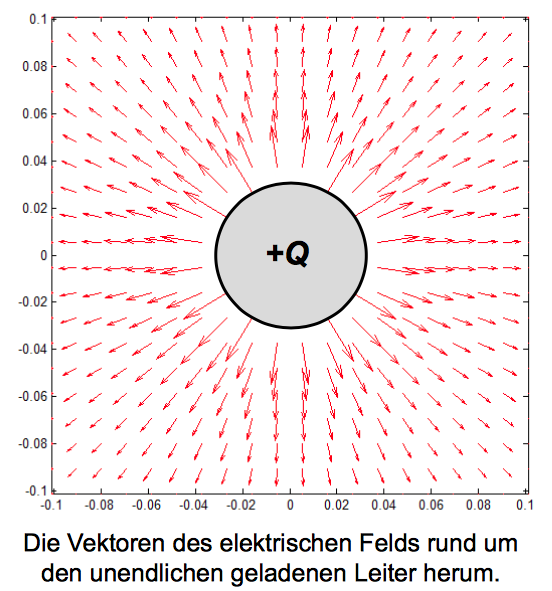
\includegraphics[width = \linewidth]{./Pics/VL1/elFeld}
\end{minipage}

\subsection{Elektrisches Potential und elektrische Spannung}

\begin{minipage}{0.5 \linewidth}
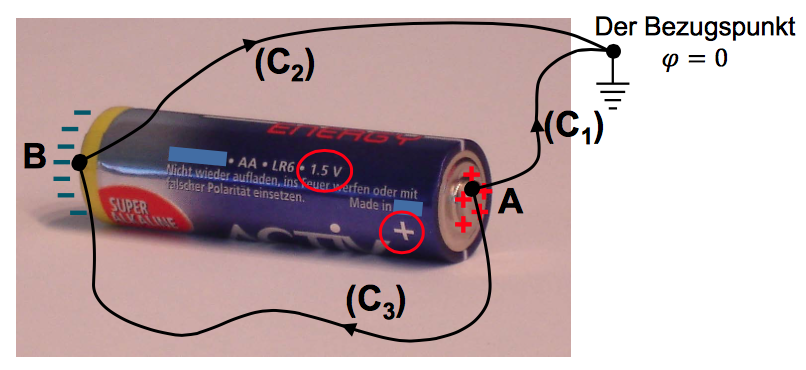
\includegraphics[width = \linewidth]{./Pics/VL1/elPot}
\end{minipage}
\begin{minipage}{0.5 \linewidth}
Die elektrische Potentiale:\\ $\varphi$ = $\int_{A}^{Bezugspunkt} \vec{E} \cdot \vec{dl}$, $\varphi_{B} = \int_{B}^{Bezugspunkt} \vec{E} \cdot \vec{dl}$
Die elektrische Spannung:
$U_{AB} = \int_{A}^{B} \vec{E} \cdot \vec{dl} = \varphi_{A} - \varphi_{B}$  (V)

Das elektrische Potential eines Ortes ist eigentlich die Arbeit, die für die Bewegung der Einheitsladung vom Bezugspunkt zum Ort nötig ist.
 \end{minipage}

\subsection{Elektrische Strom}

\begin{minipage}{0.4 \linewidth}
Elektrische Strom:

$I = \frac{dQ}{dt}$ (A)

Elektrischer Widerstand:

$R = \frac{U}{I}$  ($\Omega$)
\end{minipage}
\begin{minipage}{0.6 \linewidth}
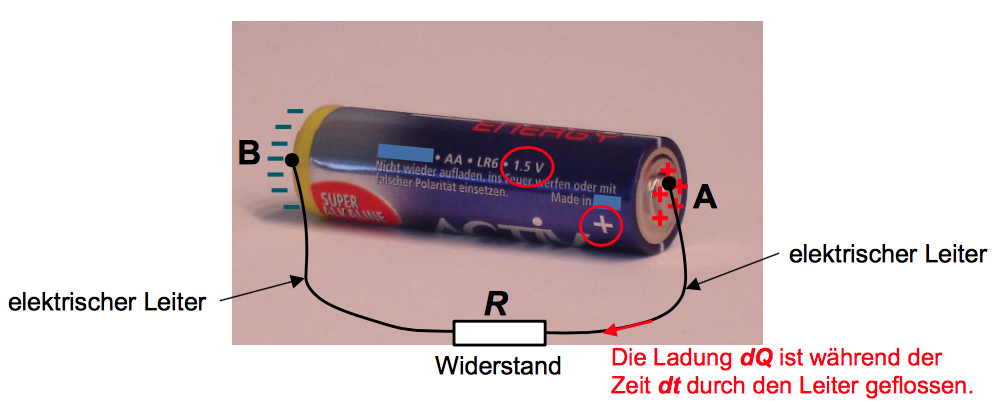
\includegraphics[width = \linewidth]{./Pics/VL1/elStrom}
 \end{minipage}
 
 \subsection{Magnetische Kraft}
 
 \begin{minipage}{0.5 \linewidth}
 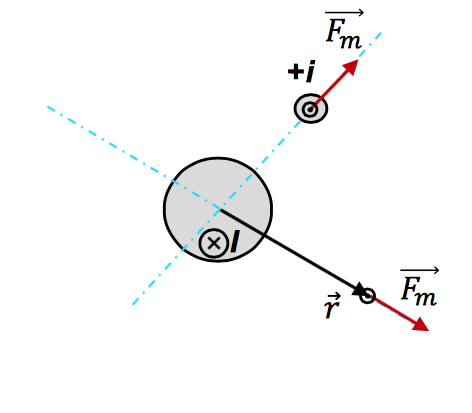
\includegraphics[width = \linewidth]{./Pics/VL1/elMag}
 \end{minipage}
 \begin{minipage}{0.5 \linewidth}
Die magnetische Kraft zwischen unendlich parallelen Leitern:
$ \vec{F_{m}} = \frac{\mu}{2 \pi} \cdot \frac{Ii}{r} \cdot \vec{r_{0}}$  ($\frac{N}{m}$) \\
$\mu$ - magnetische Permeabilität \\
$\mu_{0}$ - die Permeabilität des Vakuums \\
$\mu_{0} = 4 \pi \cdot 10^{-7}$ ($\frac{N}{A^{2}}$) \\
$I,i$ - elektrische Ströme (A) \\
$\vec{r_{0}} = \frac{\vec{r}}{|\vec{r}|} $ - Einheitsvektor \\
  \end{minipage}
  
  \begin{minipage}{0.5 \linewidth}
	Das magnetische Feld ist klein Potenzialfeld, sondern ein quellenfreies Feld: \\
	$\vec{F_{m}} = \mu \cdot i \cdot \vec{l_{0}} \times \vec{H}$  ($\frac{N}{m}$) \\
	$\vec{H} = \frac{I}{2 \pi} \cdot \frac{\vec{L_{0}} \times \vec{r_{0}}}{r}$  $(\frac{A}{m})$\\
	$\vec{r_{0}} = \frac{\vec{r}}{|\vec{r}|} $ - Einheitsvektor \\
	$\vec{L_{0}}, \vec{l_{0}}$ - Einheitsvektoren der Stromleiter \\
   \end{minipage}
   \begin{minipage}{0.5 \linewidth}
   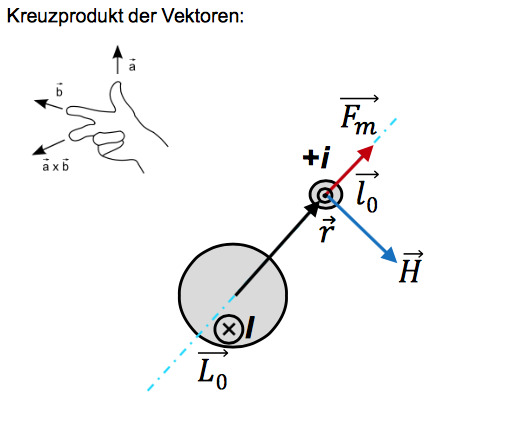
\includegraphics[width = \linewidth]{./Pics/VL1/magFeld}
    \end{minipage}
    
    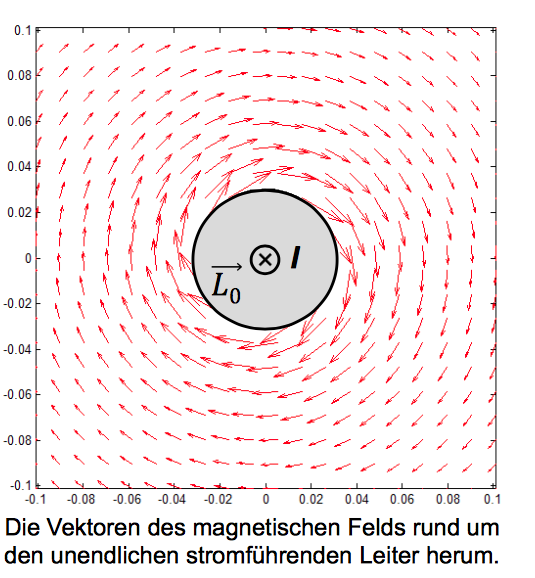
\includegraphics[width = 0.3\linewidth]{./Pics/VL1/magFeld2}
    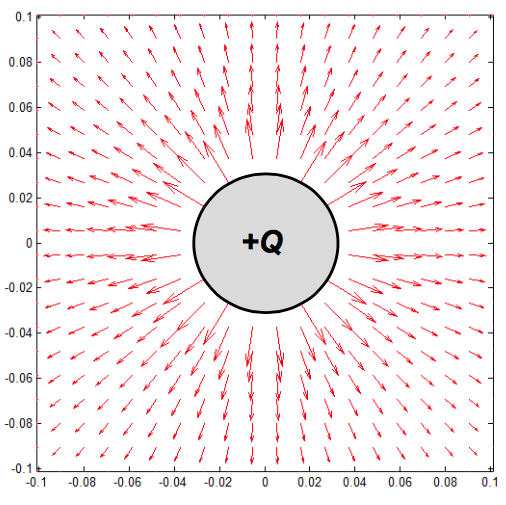
\includegraphics[width = 0.3\linewidth]{./Pics/VL1/magFeld3}
    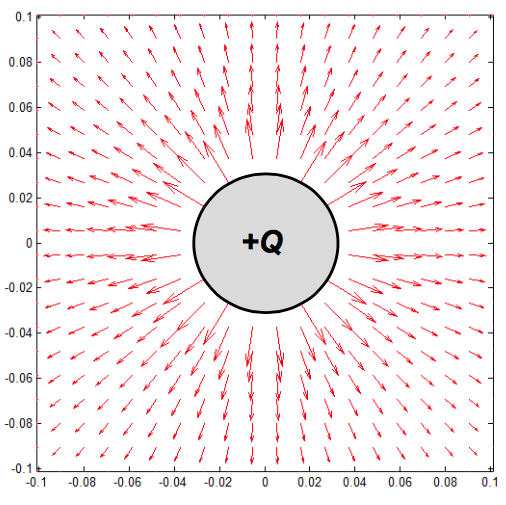
\includegraphics[width = 0.3\linewidth]{./Pics/VL1/magFeld3}
    
    $\vec{E} = \frac{1}{2 \pi \epsilon} \cdot \frac{Q}{r} \cdot \vec{r_{0}}$  ($\frac{V}{m}$) \\
    $\vec{H} = \frac{I}{2 \pi} \cdot \frac{\vec{L_{0}} \times \vec{r_{0}}}{r}$  $(\frac{A}{m})$\\
    	
\subsection{Elektrische und magnetische Kraft im Vergleich}
    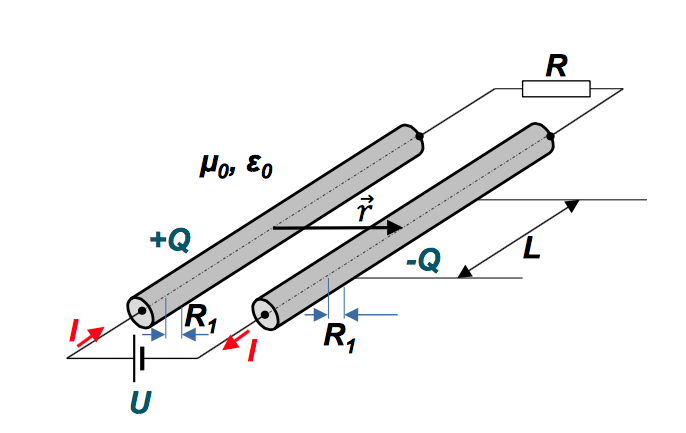
\includegraphics[width = 0.35\linewidth]{./Pics/VL1/elMagVergleich}
    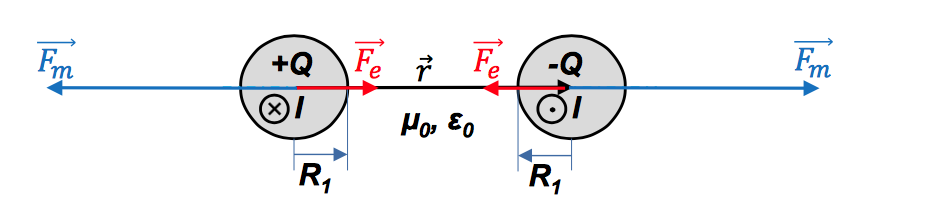
\includegraphics[width = 0.6\linewidth]{./Pics/VL1/elMagVergleich2}
    
\subsubsection{Berechnungsbeispiel}
\begin{tabular}{ll}
Die wichtige Annahme: & $r >> R_1$ \\
Die geometrischen Daten: & $R_{1}$ = 10mm, r = 100mm, L = 1000mm\\
Die elektrischen Daten:& U = 1V, I = 1A  \\
Die Kräfte pro Längeneinheit: &$F_{e} = \frac{\pi \cdot \epsilon_{0} \cdot U^{2}}{2 \cdot r \cdot (ln\frac{r-R_{1}}{R_{1}})^{2}} = 2.88 \cdot 10^{11}$ $(\frac{N}{m})$ \\
&$F_{m} = \frac{\mu_{0} \cdot I^{2}}{2 \cdot \pi \cdot r} = 2.00 \cdot 10^-6$ $(\frac{N}{m})$ \\
\end{tabular}

Die wichtigsten Schlussfolgerungen:
\begin{enumerate}
\item Der Absolutbetrag der magnetischen Kraft pro Längen- und Stromeinheit ist ungefähr $7 \cdot 10^{4}$ mal grösser als der entsprechende Betrag der elektrischen Kraft pro Längen- und Spannungseinheit.
\item Um die Kraft von 1 ($\frac{N}{m}$) in dieser Anordnung zu erzeugen ist entweder der Strom von ungefähr 700A oder die Spannung von ungefähr 600'000 V notwendig. 
\item \textbf{Die Argumente 1 und 2 deuten darauf hin, dass die magnetische Kraft für die Energieumwandlung besser als die elektrische Kraft geeignet ist.} Deswegen basieren die modernen elektrischen Maschinen hauptsächlich auf der magnetischen Kraft.
\end{enumerate}
    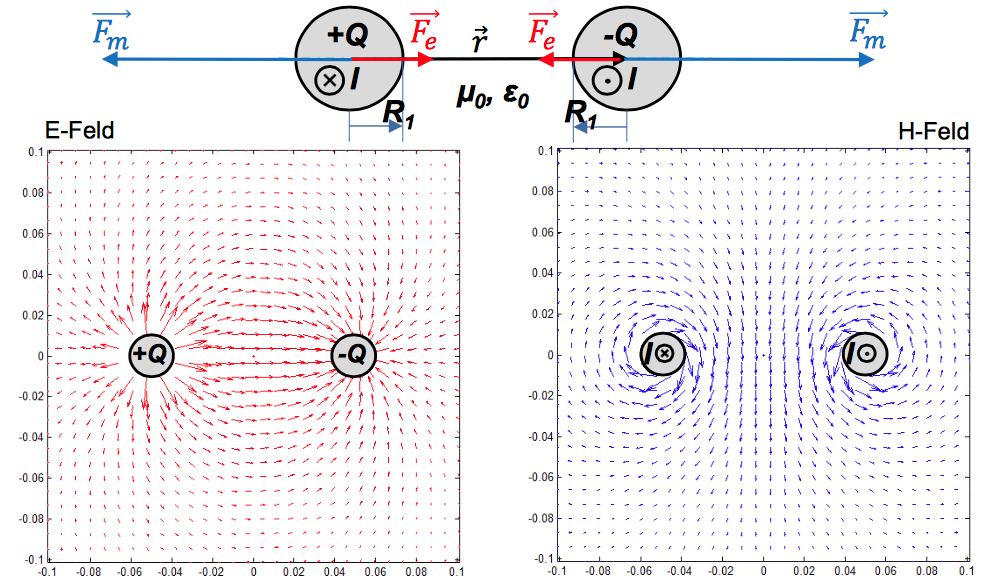
\includegraphics[width = 0.75\linewidth]{./Pics/VL1/magKraft}
    
\subsection{Begriffe und Kennwerte des Magnetfelds}
\begin{minipage}{0.2 \linewidth}
    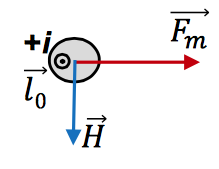
\includegraphics[width =\linewidth]{./Pics/VL1/magKraft2}
\end{minipage}
\begin{minipage}{0.8 \linewidth}
Die Kraft auf den stromführenden Leitern im Magnetfeld:\\

$\vec{F_m} = \mu \cdot i \cdot \vec{l_0} /times \vec{H}$  $(\frac{N}{m})$ = $ i \cdot \vec{l_0} \times \vec{B}$  ($\frac{N}{m}$) \\

Die magnetische Kraft ist nicht nur vom H-Feld abhängig, sondern die magnetische Eigenschaft des Materials spielen dabei auch eine wichtige Rolle. Deswegen wird \textbf{die magnetische Induktion} und \textbf{die magnetische Flussdichte} definiert:\\

$ \vec{B} = \mu \cdot \vec{H} = \mu_0 \cdot \mu_r \cdot \vec{H}$  ($T = \frac{Vs}{m^2}$) \\

$\mu_0 = 4 \pi \cdot 10^{-7}$  ($\frac{Vs}{Am} = \frac{Tm}{A}$) \\

$\mu_r = \frac{\mu}{\mu_0}$ - die relative Permeabilität des Materials \\
\end{minipage}

\begin{minipage}{0.2 \linewidth}
    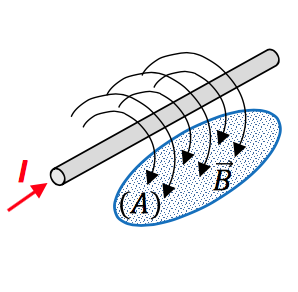
\includegraphics[width =\linewidth]{./Pics/VL1/magFluss}
\end{minipage}
\begin{minipage}{0.8 \linewidth}
\textbf{Der magnetische Fluss} ist als der Fluss des Vektors $\vec{B}$ durch eine Fläche A definiert:\\

$\Phi = \int\int_{(A)} \vec{B} \cdot \vec{dA}$ \\

Wenn der Fluss $ \Phi$ durch eine Spuhle mit $N$ Windungen fliesst, wird der gesamte Fluss der Spule denn als \textbf{der verkettete magnetische Fluss} gennant: \\

$\Psi = N \cdot \Phi$ \\

Der zeitvariierende magnetische Fluss durch eine Spule mit $N$ Windungen \textbf{induziert die folgende elektrische Spannung} in der Spule.\\

$U_{ind} = - \frac{d \Psi}{dt} = -N \frac{d \Phi}{dt}$ (V)
\end{minipage}

\begin{minipage}{0.2 \linewidth}
    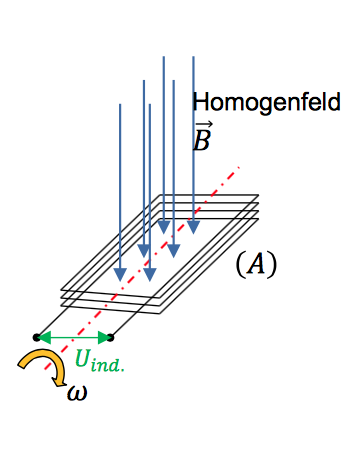
\includegraphics[width =\linewidth]{./Pics/VL1/elGen}
\end{minipage}
\begin{minipage}{0.8 \linewidth}
\textbf{Das Wirkungsprinzip eines elektromagnetischen Generators} ist hier dargestellt. Der Generator besteht im Wesentlichen aus einer Spule mit $N$ Windungen, die sich im magnetischen Homogenfeld um ihre Achse mit der konstanten Winkelgeschwindigkeit $\omega$ dreht:\\

$\Psi (t) = N \cdot \int\int_{(A)} \vec{B} \cdot \vec{dA} = N \cdot B \cdot A \cdot cos(\omega t) $ \\

\textbf{Die induzierte Spannung} der Spule kann wie folgt gerechnet werden: \\

$U_{ind.} = - \frac{d\Psi}{dt} = \omega \cdot N \cdot B \cdot A \cdot sin(\omega t)$  $(V)$
\end{minipage}

\subsection{Zusammenfassung}

\begin{itemize}
\item Die elektrische Kraft wirkt auf eine elektrische Ladung im elektrsichen Fremdfeld.
\item Die magnetische Kraft wirkt auf einen stromführenden Leiter im magnetischen Fremdfeld.
\item Die magnetische Kraft zwischen zwei parallelen stromdurchflossenen Leitern pro Strom- und Längeneinheit ist viel höher als die entsprechende elektrische Kraft zwischen den Leitern pro Spannung- und Längeneinheit.
\item Der elektrische Wechselstrom erzeugt das magnetische Wechselfeld.
\item In einer Spule, die sich im magnetischen Wechselfeld befindet, wird die elektrische Wechselspannung induziert.
\end{itemize}
\section{Magnetkreis-Begriff, Permanentmagnet, Reluktanzkraft}
\subsection{Magnetische Durchflutung}
\begin{minipage}{0.2 \linewidth}
    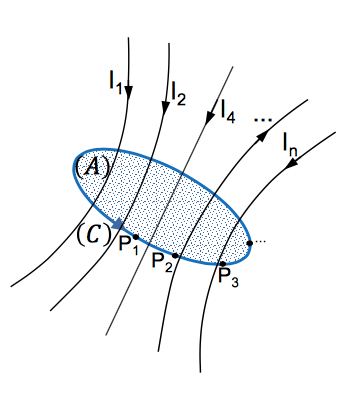
\includegraphics[width =\linewidth]{./Pics/VL2/magDurchflutung}
\end{minipage}
\begin{minipage}{0.8 \linewidth}
\textbf{Die magnetische Durchflutung} einer von der Kontur (C) umrandetetn Fläche (A) ist der gesamte Strom, der durch diese Fläche fliesst: \\

$\Theta = \sum_{k = 1}^{n} I_k$\\

Nach dem \textbf{Durchflutungsgesetz} muss das Linienintegral des magnetischen Felds entlang der Kontur (C) die entsprechende elektrische Durchlutung ergeben: \\

$\oint \vec{H} \cdot \vec{dl} = \sum_{k=1}^{n} I_k = \Theta$\\

Diese Gleichung ist eine sehr wichtige Verknüpfung zwischen dem Magnetfeld und dem elektrischen Strom. Sie wird sehr oft \textbf{für die Berechnung des Magnetfelds} einer angegebenen Erreger-Anordnung eingesetzt. 
\end{minipage}
\subsection{Magnetische Spannung}
\begin{minipage}{0.2 \linewidth}
    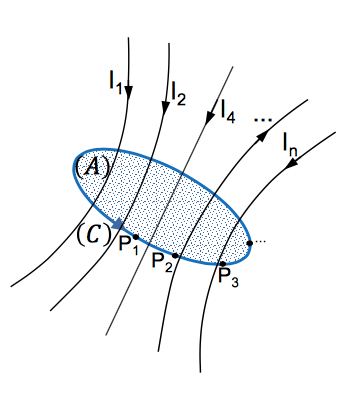
\includegraphics[width =\linewidth]{./Pics/VL2/magDurchflutung}
\end{minipage}
\begin{minipage}{0.8 \linewidth}
Um das Linienintegral einfacher zu rechnen sollte die Integrationskurve (C) passen definiert und aufgeteilt werden: \\

$\oint_{(C)} \vec{H} cdot \vec{dl} = \oint_{P_1}^{P_2} \vec{H} \cdot \vec{dl} + \oint_{P_2}^{P_3} \vec{H} \cdot \vec{dl}  + \cdots +\oint_{P_{m-1}}^{P_m} \vec{H} \cdot \vec{dl} $ \\

Der Definition der elektrischen Spannung zufolge, wird die magnetische Spannung wie folgt definiert: \\

$V_m = \int^B_A \vec{H} \cdot \vec{dl}$ \\

Die Aufteilung der Integrationskurve(C) wird normalerweise so durchgeführt, dass eine Summation anstatt der Integration ergeben wird: \\

$\oint_{(C)} \vec{H} \cdot \vec{dl} = H_1 \cdot l_1 + H_2 \cdot l_2 + H_3 \cdot l_3 + \cdots = V_{m1} + V_{m2} + V_{m3} + \cdots$
\end{minipage}

\subsection{Magnetischer Widerstand}
\begin{minipage}{0.2 \linewidth}
    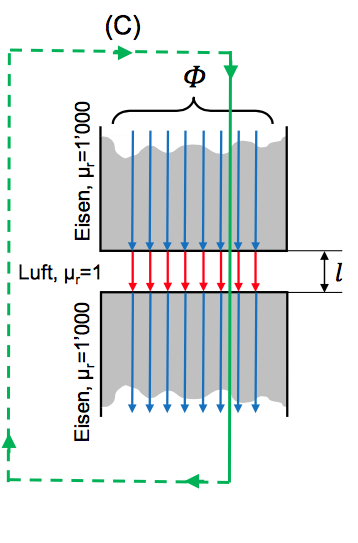
\includegraphics[width =\linewidth]{./Pics/VL2/magR}
\end{minipage}
\begin{minipage}{0.8 \linewidth}
Der magnetische Fluss durch einen Luftspalt zwischen den Eisenblöcken lässt sich wie folgt angeben:\\

$\Phi_{1Eisen} = \Phi_{Luft} = \Phi_{2Eisen} \Rightarrow B_{1Eisen} =  B_{Luft} = B_{2Eisen}$ \\

Jedoch ist die magnetische Permeabilität von Eisen etwa 1000 mal grösser als die Permeabilität von Luft, was in dieser Anordnung das magnetische Feld im Luftspalt bestimmt: \\

$B_{1Eisen} = B_{Luft} \Rightarrow \mu_{0} \cdot \mu_{rEisen} \cdot H_{Eisen} = \mu_0 \cdot \mu_{rLuft} \cdot H_{Luft}$ \\

$H_{Luft} = \frac{\mu_{rEisen}}{\mu_{rLuft}} \cdot H_{Eisen} \Rightarrow H_{Luft} \approx 1'000 \cdot H_{Eisen}$ \\

Offenbar ist das magnetische Feld in der Luft viel grösser als das entsprechende Feld im Eisen. Das bedeutet, dass die magnetische Spannung entlang einer Flusslinie mit den Luftstrecken der Linie bestimmt wird: \\

$\oint_{(C)} \vec{H} \cdot \vec{dl} = H_{Eisen} \cdot l_{Eisen} + H_{Luft} \cdot l_{Luft} \approx H_{Luft} \cdot l_{Luft} = V_{mLuft}$ \\

Die magnetische Spannung des Luftspalts spielt eine wichtige Rolle in jeder Anordnung mit einem Eisenkern: \\

$\oint_{(C)} \vec{H} \cdot \vec{dl} \approx H_{Luft} \cdot l_{Luft} = V_{mLuft}$ \\

Der Definition des elektrischen Widerstands zufolge, wird den magnetischen Widerstand wie folgt definiert: \\

$R_m = \frac{V_m}{\Phi}$ \\

Wenn $A$ die auf den magnetischen Fluss senkrechte Fläche des Luftspaltes ist, lässt sich denn der magnetische Widerstand des Luftspaltes wie folgt angeben: \\

$R_m = \frac{H_0 \cdot l}{B_0 \cdot A} = \frac{H_0 \cdot l}{\mu_0 \cdot H_0 \cdot A} = \frac{l}{\mu_0 \cdot A}$
 \end{minipage}

\subsection{Magnetkreis}

Die Annahme der Feldberechnung: \\
Das magnetische Feld in der Spule ist \textbf{viel grösser} als draussen und das Feld in der Spule \textbf{ist homogen}. Die Annahmen sind dann realistisch, wenn $L >> R$ ist.\\

$\oint_{(C)} \vec{H} \cdot \vec{dl} \approx H \cdot L = N \cdot I \Rightarrow H = \frac{N \cdot I}{L}, B = \mu_0 \cdot \frac{N \cdot I}{L}$

\begin{minipage}{0.5 \linewidth}
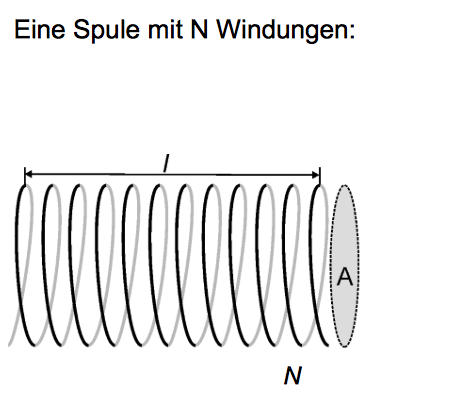
\includegraphics[width = \linewidth]{./Pics/VL2/spule}
\end{minipage}
\begin{minipage}{0.5 \linewidth}
Das magnetische Feld und die magnetische Flussdichte der Spule: \\

$H = \frac{N \cdot I}{L}$ \\

Für die Spule mit den folgenden geometrischen Daten: \\

R = 0.1m, L = 0.27m, N = 10, I = 1A \\

wird das folgende magnetische Feld gerechnet: \\

$H = 37.4 \frac{A}{m}, B = 46.5 \mu T $\\

$\mu_0 = 4 \pi \cdot 10^{-1}$ ($\frac{Tm}{A}$)
\end{minipage}

\subsubsection{H-Feld im Luftspalt (vereinfachte Herleitung)}
\begin{minipage}{0.4 \linewidth}
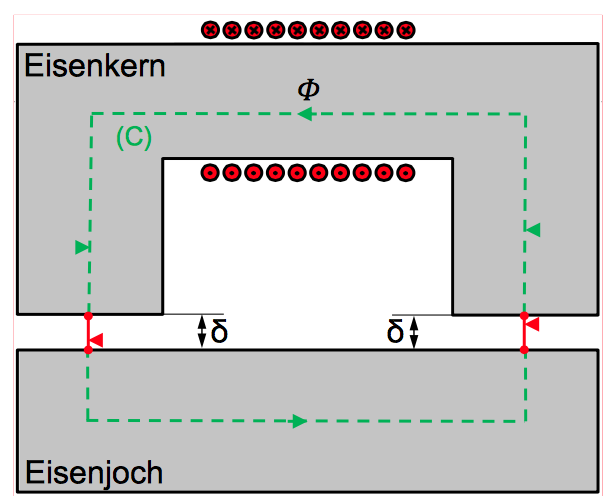
\includegraphics[width = \linewidth]{./Pics/VL2/magKreis}
\end{minipage}
\begin{minipage}{0.6 \linewidth}
Gemäss dem Durchflutungsgesetz lässt sich das Magnetfeld eines Magnetkreises wie folgt angeben: \\

$\oint_{(C)} \vec{H} \cdot \vec{dl} = H_{Fe} \cdot l_{Fe} + 2 \cdot \delta \cdot H_{\delta}  = I \cdot N $ \\

Wie schon präsentiert, ist in dieser Anordnung das magnetische Feld im Luftspalt viel grösser als das entsprechende Feld im Eisen: \\

$H_{\delta} \approx \cdot H_{Fe} \Rightarrow H_{\delta} = \frac{I \cdot N}{2 \delta} $ \\

$B_{\delta} = \mu_0 \frac{I \cdot N}{2 \delta} $ \\

Ein Magnetkreis mit einer stromdurchflossenen Spule erzeugt einen magnetischen Fluss, der den entsprechenden Magnetfluss ohne Magnetkreis mehrere Grössenordnungen überschiesst. 
\end{minipage}

\subsubsection{Beispiele}
\includegraphics[width = 0.8 \linewidth]{./Pics/VL2/magKreisBeispiele}

\subsubsection{H-Feld im Luftspalt (Allgemeine Herleitung)}
\begin{minipage}{0.4 \linewidth}
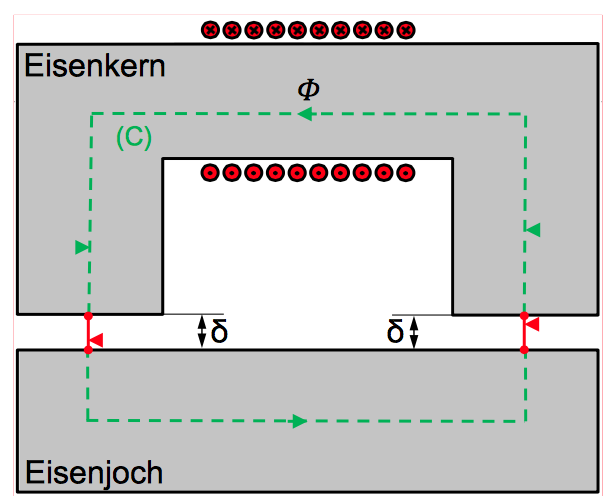
\includegraphics[width = \linewidth]{./Pics/VL2/magKreis}
\end{minipage}
\begin{minipage}{0.6 \linewidth}
Wenn der Magnetkern in der Stättigung ist, lässt sich das H-Feld im Eisen nicht mehr vernachlässigen: \\

$\oint_{(C)} \vec{H} \cdot \vec{dl} = H_{Fe} \cdot l_{Fe} + 2 \cdot \delta \cdot H_{\delta} $ \\

$H_{Fe} \cdot l_{Fe} + 2 \delta \cdot H_{\delta} = I \cdot N$ \\

$\Phi_{\delta} = \Phi_{Fe} \Rightarrow B_{\delta} = B_{Fe}$ \\

$H_{Fe} = \frac{B_{Fe}}{\mu_{Fe}} = \frac{B_{\delta}}{\mu_{Fe}} = \frac{\mu_0}{\mu_{Fe}} \cdot H_{\delta}$\\

$\frac{\mu_0}{\mu_{Fe}} \cdot H_{\delta} \cdot l_{Fe} + 2 \cdot \delta \cdot H_{\delta} = I \cdot N$\\

\textbf{$H_{\delta} = \frac{I \cdot N}{\frac{\mu_0}{\mu_{Fe}}+ 2 \delta}$}
\end{minipage}

\subsection{Permanentmagnet}

\begin{minipage}{0.3 \linewidth}
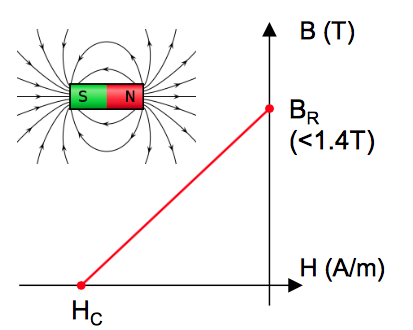
\includegraphics[width = \linewidth]{./Pics/VL2/permanentMagnet}
\end{minipage}
\begin{minipage}{0.7 \linewidth}
Ein Permanentmagnet (Dauermagnet) ist ein Stück eines magnetisierbaren Materials (Eisen, Kobalt, Nickel, Ferrit) welches sein statisches Magnetfeld behält ohne einen elektrischen Stromfluss. \\

Kennwerte der Dauermagnete:
\begin{itemize}
\item \textbf{Koerzitivfeldstärke $H_c$} Dieses Magnetfeld muss erzeugt werden um den Dauermagneten vollständig zu entmagnetisieren (B=0)
\item \textbf{Remanenz $B_R$} Das ist die magnetische Flussdichte des Dauermagnets ohne magnetisches Fremdfeld (H=0)
\item $B_m = \mu_m \cdot H_m + B_R , \mu_m = \mu_0$
\end{itemize}

Die Permanentmagneten ersetzen die Erregerspulen in den elektrischen Maschinen. Damit sind die Materialkosten und die ohmschen Verluste der Erregerspulen eliminiert. 
\end{minipage}

\subsubsection{Magnetkreis mit einem Dauermagneten (Allg. Herleitung)}
\begin{minipage}{0.4 \linewidth}
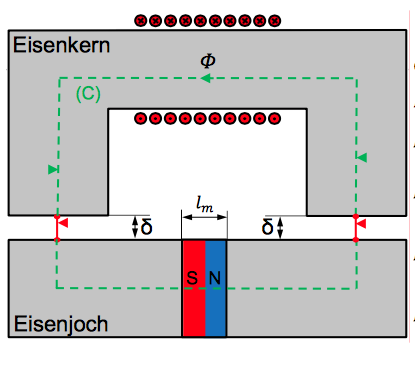
\includegraphics[width = \linewidth]{./Pics/VL2/permMagnet}
\end{minipage}
\begin{minipage}{0.6 \linewidth}
$\oint_{(C)} \vec{H} \cdot \vec{dl} = H_{Fe} \cdot l_{Fe} + H_{m} \cdot l_{m} + 2 \cdot \delta \cdot H_{\delta} $ \\

$H_{Fe} \cdot l_{Fe} + H_{m} \cdot l_{m} + 2 \cdot \delta \cdot H_{\delta} = I \cdot N$ \\

$B_m = B_\delta = B_{Fe}$ \\

$B_m = \mu_m \cdot H_m + B_R \Rightarrow H_m = \frac{B_m - B_R}{\mu_m}$ \\

$H_m =  \frac{\mu_0 \cdot H_\delta  - B_R}{\mu_m}$\\

$H_{Fe} = \frac{B_{Fe}}{\mu_{Fe}} = \frac{\mu_0}{\mu_{Fe}} \cdot H_\delta$\\

$H_m = \frac{\mu_0 \cdot H_\delta - B_R}{\mu_m}$\\

$H_{Fe} = \frac{B_{Fe}}{\mu_{Fe}} = \frac{\mu_0}{\mu_{Fe}}\cdot H_\delta $ \\

$\frac{\mu_0}{\mu_{Fe}} \cdot H_\delta \cdot l_{Fe} + \frac{\mu_0 \cdot H_\delta - B_R}{\mu_m} \cdot l_m + 2 \cdot \delta \cdot H_\delta = I \cdot N$

$H_\delta = \frac{I \cdot N + \frac{B_R}{\mu_m} \cdot l_m}{\frac{\mu_0}{\mu_{Fe}} \cdot l_{Fe} + \frac{\mu_0}{\mu_m} \cdot l_m + 2 \cdot \delta}$
\end{minipage}


\subsection{Reluktanzkraft}
\begin{minipage}{0.4 \linewidth}
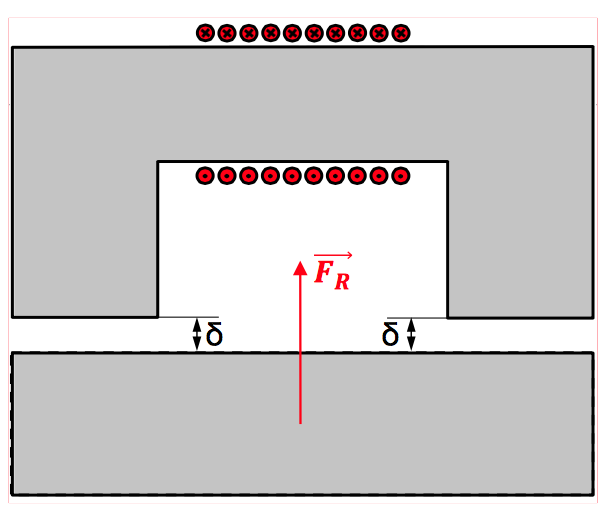
\includegraphics[width = \linewidth]{./Pics/VL2/reluktanz}
\end{minipage}
\begin{minipage}{0.6 \linewidth}
Die ferromagnetischen Körper sind im magnetischen Fremdfeld der so genannten Reluktanzkraft ausgesetzt. \\

Die Reluktanzkraft wirkt auf die ferromagnetischen Körper nur anziehen. \\

In dieser Anordnung lässt sich die Reluktanzkraft so angeben: \\

$F_R  = \mu_0 \frac{N^2 \cdot I^2 \cdot A}{4 \delta^2}$ \\

wobei A die magnetisch wirksame Fläche des Luftspalts ist. \\

Die magnetische Energie:\\

$W_m = \frac{1}{2} \cdot H_\delta \cdot B_\delta \cdot 2 \cdot A_{Fe} \cdot \delta= \mu_0 \cdot \frac{I^2 \cdot N^2}{4 \cdot \delta} \cdot A_{Fe}$ \\ 

wobei $A_{Fe} \cdot \delta$ das Volumen des Luftspalts ist. \\

Die Reluktanzkraft nach der Methode der virtuellen Verrückung: \\

$F_R = - \frac{\eth W_m}{\eth \delta} = \mu_0 \frac{I^2 \cdot N^2}{4 \cdot \delta^2} \cdot A_{Fe}$
\end{minipage}

\subsection{Zusammenfassung}

\begin{itemize}
\item Das magnetische Durchflutungsgesetz wird häufig für die Magnetfeldberechnung der stromdurchflossenen Spulen mit und ohne Magnetkreis eingesetzt. 
\item Ein Magnetkreis mit einer stromdurchflossenen Spule erzeugt einen magnetischen Fluss, der den entsprechenden Magnetfluss ohne Magnetkreis mehrere Grössenordnungen überschiesst.
\item Die magnetische Stromkraft wirkt auf einen stromführenden Leiter in einem fremden Magnetfeld.
\item Die magnetische Reluktanzkraft wirkt auf einen ferromagnetischen Körper im fremden Magnetfeld.
\item Die Permanentmagneten ersetzten stromdurchflossene Erregerspulen in den elektrischen Maschinen. Damit werden die Materialkosten und die ohmschen Verluste der Errgerspule eliminiert.
\end{itemize}
\section{Gleichstrommaschine (GSM)}
\subsection{Einleitung}
\begin{itemize}
\item Gleichstrommaschinen werden bis ca. 3kV Nennspannung und bis zu einer Leistung von 20 MW hergestellt.
\item Gleichstrommaschinen werden heute häufig in dynamischen Bereichen, mit ständig ändernden Drehzahlen in weiten Bereichen eingesetzt.
\end{itemize}

\subsection{Aufbau und Wirkungsprinzip}
\begin{minipage}{0.5 \linewidth}
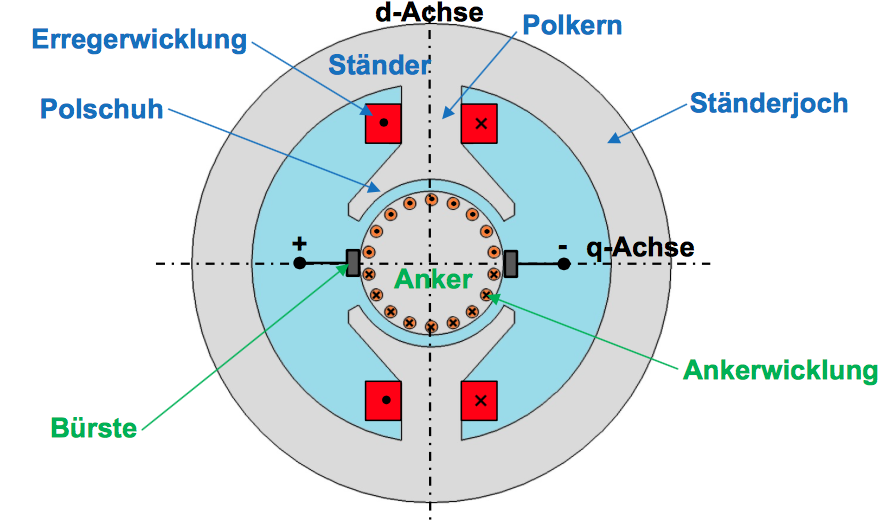
\includegraphics[width = \linewidth]{./Pics/VL45/GSMAufbau}
\end{minipage}
\begin{minipage}{0.5 \linewidth}
\begin{itemize}
\item Die vom Gleichstrom durchflossene Erregerwicklung erzeugt das magnetische Hauptfeld der Maschine.
\item Das Ständerjoch, der Polkern, der Polschuh und der Ankerkern sind aus lamelliertem Eisen gefertigt, weil Eisen magnetische Feldlinien viel besser als Luft ($\mu_{rFE} \approx 10^5$) führt. 
\item Der magnetische Fluss fliesst durch den Kern des Ständers, überspringt den Luftspalt zwischen dem Polschuh und Rotor und geht weiter durch den Kern des Rotors.
\item \textbf{Gleichstromgenerator:} Durch die Umdrehung der Ankerwicklung im magnetischen Hauptfeld wird die Wechselspannung in den Wicklungen induziert. Die Induzierte Spannung der Ankerwicklung wird mit den Bürsten und Schleifringen (Kommutator) gleichgerichtet und nach aussen geführt.
\item \textbf{Gleichstrommotor:} Eine Gleichstromquelle wird über den Kommutator mit den Ankerwicklungen verbunden. Wenn der elektrische Strom durch die Ankerwicklung im magnetischen Hauptfeld fliesst, wird denn die auf die Ankerwicklung wirkende magnetische Kraft (d.h. das Moment des Motors) erzeugt. 
\end{itemize}
\end{minipage}

\subsubsection{Wirkungprinzip GSM-Motor}
Wenn der elektrische Strom durch die Ankerwicklung im magnetischen Hauptfeld fliesst, wird die auf die Ankerwicklung wirkende magnetische Kraft (d.h. das Moment des Motors) erzeugt:

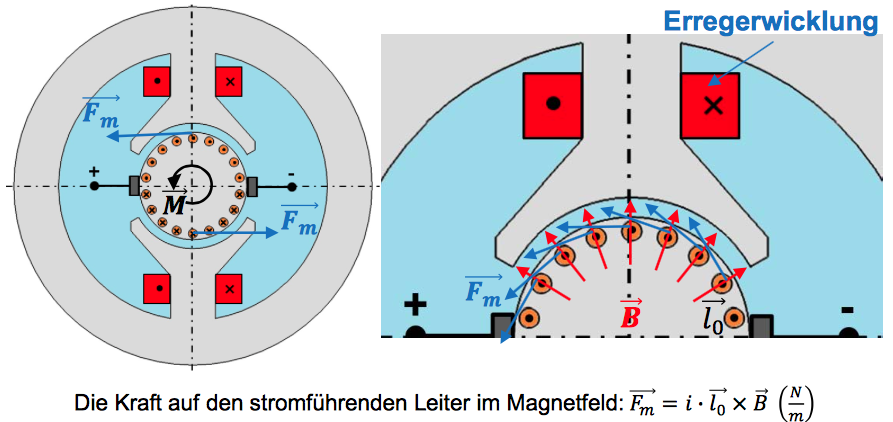
\includegraphics[width = 0.8 \linewidth]{./Pics/VL45/GSMMotor}

\subsection{Grundgleichungen, Kommmutierung, Ersatzschaltbild}
\begin{minipage}{0.3 \linewidth}
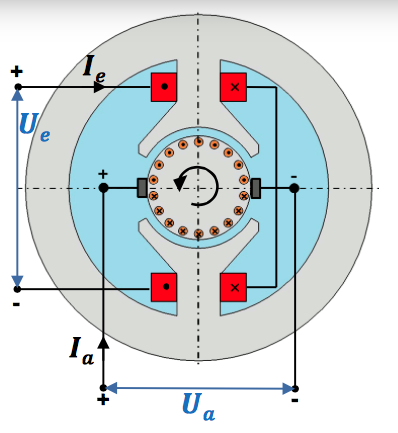
\includegraphics[width = \linewidth]{./Pics/VL45/GSM}
\end{minipage}
\begin{minipage}{0.6\linewidth}
Die Erregerwicklung, die den Erregerwiderstand $R_e$ und die Erregerinduktivität $L_e$ besitzt, wird an die Spannungsquelle $U_e$ angeschlossen. Gemäss dem zweiten Kirchooffschen Gesetz sind die Erregerspannung $U_e$ und der Erregerstrom $I_e$ wie folgt verknüpft: \\

$U_e = R_e \cdot I_e + L_e \cdot \frac{dI_e}{dt}$ \\

Ebenso weisst die Ankerspule im Läuferkreis den Ankerwiderstand $R_a$ und die Ankerinduktivität $L_a$ auf. Im Gegensatz zu der Erregerwicklung dreht sich die Ankerspule im magnetischen Hauptfeld um und dadurch wird in dieser Spule eine zusätzliche Spannung $E$ induziert, die im Ankerkreis eine wichtige Rolle spielt: \\

$U_a = R_a \cdot I_a + L_a \cdot \frac{dI_a}{dt} + E$
\end{minipage}

\begin{minipage}{0.25 \linewidth}
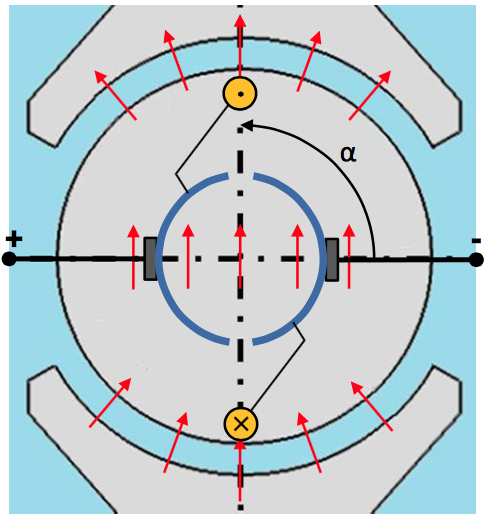
\includegraphics[width = \linewidth]{./Pics/VL45/GSM2}
\end{minipage}
\begin{minipage}{0.7\linewidth}
\begin{itemize}
\item Um die Kommutierung des Ankerstroms zu erklären ist nur eine Anker-Leiterschleife (gelb) dargestellt. Die beiden Enden der Schleife sind mit den zwei seperaten Schleifringen (blau) verbunden. Die Schleifringe zusammen mit den anliegenden Bürsten werden als Kommutator oder Stromwender gennant.
\item Die Stromführung zwischen dem äusseren elektrischen System und den rotierenden Ankerspulen ermöglichen die durch Federdruck gepressten Kohlebürsten.
\end{itemize}
\end{minipage}


\begin{minipage}{0.4 \linewidth}
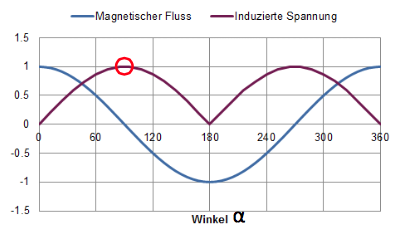
\includegraphics[width = \linewidth]{./Pics/VL45/GSM3}
\end{minipage}
\begin{minipage}{0.6\linewidth}
Die Position der Bürsten ist sehr wichtig für die verlustfreie Kommutierung. Wenn eine Bürste gleichzeitig die beiden Schleifringe berührt ($\alpha = 180\degree$), muss in diesem Moment die induzierte Spannung der entsprechenden Wicklungsektion gleich Null werden. Sonst werden Lichtbögen zwischen den Lamellen des Kommutators entstanden, was als Läuferfeuer bekannt ist. Das Läuferfeuer ist ein klares Anzeichen der schlechten Kommutierung, die die Lebensdauer der Maschine wesentlich verkürzen könnte.
\end{minipage}

\subsection{Ersatzschaltbild}
\begin{minipage}{0.4 \linewidth}
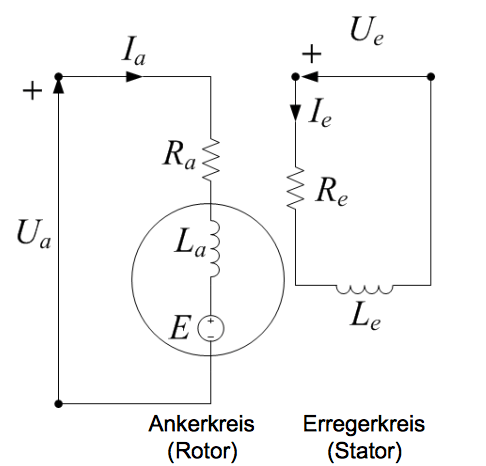
\includegraphics[width = \linewidth]{./Pics/VL45/GSMErsatzschaltbild2}
\end{minipage}
\begin{minipage}{0.6\linewidth}
Die Spannungsgleichung des Statorkreises: \\

$U_e = R_e \cdot I_e + L_e \cdot \frac{dI_e}{dt}$ \\

Die Spannungsgleichung des Rotorkreises: \\

$U_a = R_a \cdot I_a + L_a \cdot \frac{dI_a}{dt} + E $\\

Die induzierte Spannung der Ankerwicklung lässt sich so angeben: \\

$E = \omega \cdot \Psi$\\

wobei $\omega = 2 \cdot \pi \cdot n / 60$ die Winkelgeschwindigkeit des Läufers, $n$ die Drehzahl des Läufers, und $\Psi$ der verkettete Erregerfluss ist. 
\end{minipage}

\subsection{Drehmoment}
\begin{minipage}{0.4 \linewidth}
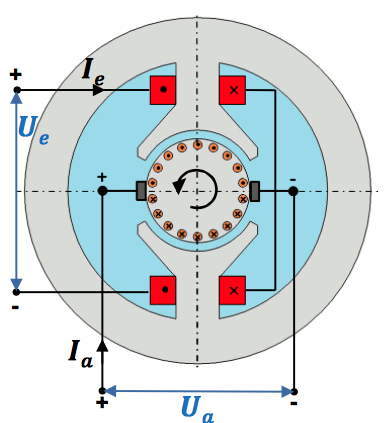
\includegraphics[width = \linewidth]{./Pics/VL45/GSMErsatzschaltbild}
\end{minipage}
\begin{minipage}{0.6 \linewidth}
Die elektrische Leistung der Maschine im stationären Betrieb ($\frac{d}{dt} = 0$) lässt sich wie folgt angeben: \\

$P_{el} = P_e + P_a = U_e \cdot I_e + U_a \cdot I_a$ ($W$) \\

$P_{el} = R_e \cdot I_e^2 + R_a \cdot I_a^2 + \omega \cdot \Psi \cdot I_a$ ($W$) \\

$R_e \cdot I_e^2$  - Ohmsche Erregerverluste \\

$R_a \cdot I_a^2$  - Ohmsche Ankerverluste \\

$\omega \cdot \Psi \cdot I_a$ -  Mechanische Leistung \\

$P_mech = \omega \cdot M$ ($W$), wobei M das Drehmoment ist. \\

$M = \Psi \cdot I_a$ ($Nm$)
\end{minipage}

\subsection{Ankerrückwirkung}
\begin{minipage}{0.4 \linewidth}
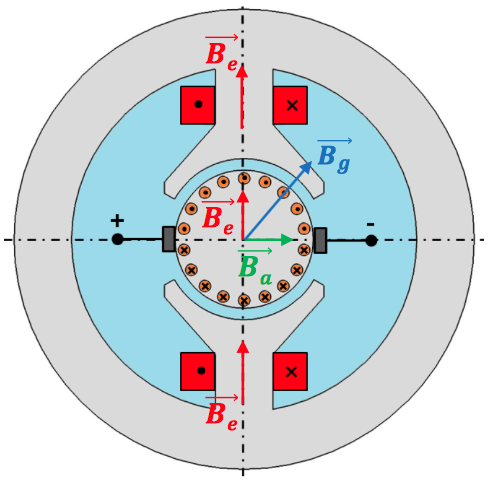
\includegraphics[width = \linewidth]{./Pics/VL45/Ankerruek}
\end{minipage}
\begin{minipage}{0.6 \linewidth}
Der Ankerstrom erzeugt sein eigenes magnetisches Feld, das die Symmetrie des Erregerfelds deutlich verzerrt. Dieser Effekt ist als die Ankerrückwirkung bekannt. \\

Das Gesamtfeld wird durch die Vektoraddition gerechnet: \\

$\vec{B_g} = \vec{B_e} + \vec{B_a}$ ($T$)
\end{minipage}

\begin{minipage}{0.6 \linewidth}
\begin{itemize}
\item Die vom Gleichstrom durchflossene Erregerwicklung erzeugt das magnetische Hauptfeld der Maschine.
\item Die Ständerwicklung und der magnetische Kern der Maschine sind sehr symmetrisch. Deswegen sind die B-Feldlinien über die Geometrie das Maschine auch gleichmässig und symmetrisch verteilt. 
\end{itemize}
\end{minipage}
\begin{minipage}{0.4 \linewidth}
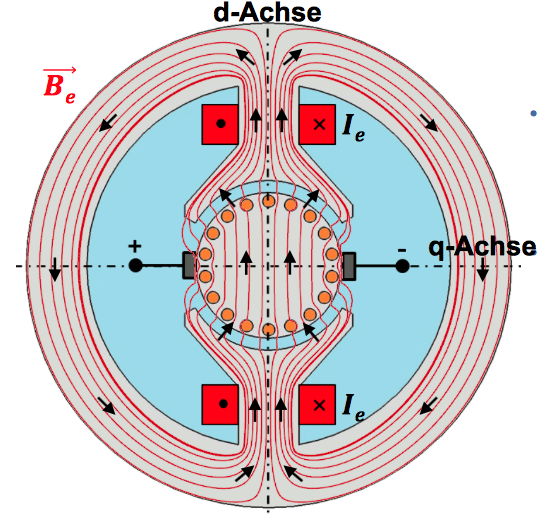
\includegraphics[width = \linewidth]{./Pics/VL45/Ankerruek2}
\end{minipage}

\begin{minipage}{0.4 \linewidth}
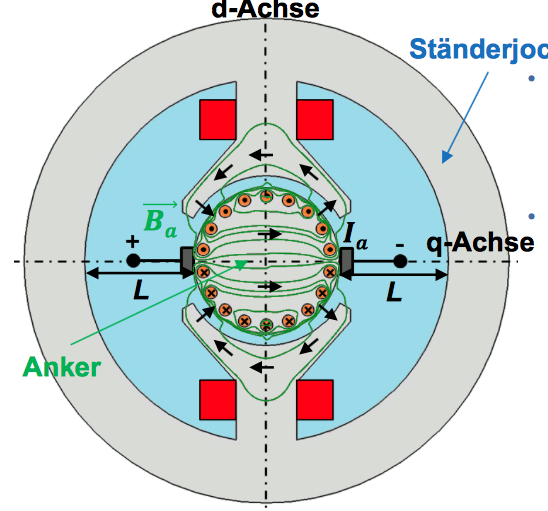
\includegraphics[width = \linewidth]{./Pics/VL45/Ankerruek3}
\end{minipage}
\begin{minipage}{0.6 \linewidth}
\begin{itemize}
\item Der Ankerstrom erzeugt das eigene magnetische Feld, das im Ankerkern parallel zu der q-Achse ausgerichtet ist. 
\item Da in der Richtung der q-Achse der Abstand (L) zwischen dem Anker und dem Ständerjoch sehr gross ist, finden die magnetischen Feldlinien den Rückweg entweder zwischen der Ankerwicklung und der äusseren Ankerfläche (sehr eng) oder durch den Luftspalt und den Polschuh (realtiv breit).
\end{itemize}
\end{minipage}

\begin{minipage}{0.6 \linewidth}
\begin{itemize}
\item Die Wirkung des Ankerfelds ist im Anker und im Luftspalt offenbar am stärksten.
\item Die Verzerrung des magnetischen Gesamtfelds im Anker löst die Verschiebung des Winkels aus, der dem Nulldurchgang der induzierten Ankerspannung entspricht.
\item Wenn der Winkel des Nulldurchgangs der induzierten Nullspannung und die Position der Bürsten nicht übereinander liegen, werden die schlechte Kommutierung und dadurch das Läuferfeuer ausgelöst.
\end{itemize}
\end{minipage}
\begin{minipage}{0.4 \linewidth}
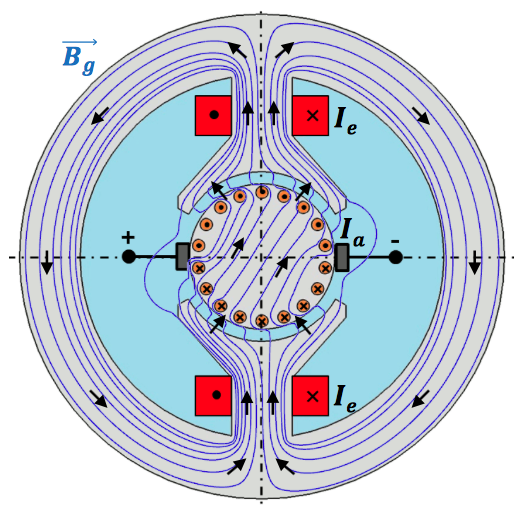
\includegraphics[width = \linewidth]{./Pics/VL45/Ankerruek4}
\end{minipage}

\subsubsection{Kompoundwicklung}
\begin{minipage}{0.4 \linewidth}
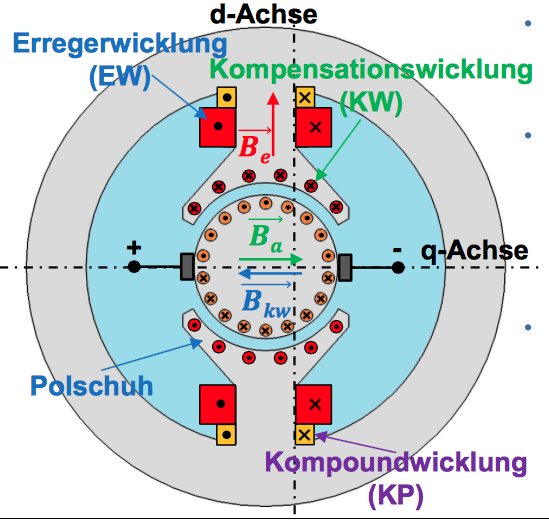
\includegraphics[width = \linewidth]{./Pics/VL45/Kompoundwicklung}
\end{minipage}
\begin{minipage}{0.6 \linewidth}
\begin{itemize}
\item Um die Rückwirkung des Ankerwicklung zu vermindern, wird eine zusätzliche Wicklung, die als Kompensationswicklung (KW)  bekannt ist, im Polshuh des Stators eingesetzt.
\item Der Strom der KW-Wicklung ist so ausgesetzt, dass dessen magnetisches Feld ($B_{kw}$) das Feld der Ankerwicklung aufhebt.
\item Die KW-Wicklung ist konstruktiv sehr aufwändig und damit auch teuer. Deswegen wird sie nur bei Hochleistungsmaschinen verwendet.
\item Die Nuten der KW-Wicklung reduzieren das Hauptfeld $B_e$ (Luft statt Eisen).
\item Um die durch die KW-Wicklung verursachte Hauptfeldschwächung zu kompensieren, wird die Kompoundwicklung (KP) eingesetzt. 
\item Die Hauptfeldkompensation sollte lastabhängig sein. Deswegen fliesst der Ankerstrom auch durch die KP-Wicklung (Reihenschaltung). 
\end{itemize}
\end{minipage}

\subsubsection{Wendepolwicklung}
\begin{minipage}{0.6 \linewidth}
\begin{itemize}
\item Um das Feldverzerrung in der geometrisch neutralen Zone (q-Achse) bei Laständerung zu minimieren und dadurch die Qualität der Kommutierung zu verbessern, wird die Wendepolwicklung (WW) eingesetzt. 
\item Die Wendepolwicklung wird vom Ankerstrom durchflossen, weil die Wirkung der WW-Wicklung lastabhängig sein muss.
\end{itemize}
\end{minipage}
\begin{minipage}{0.4 \linewidth}
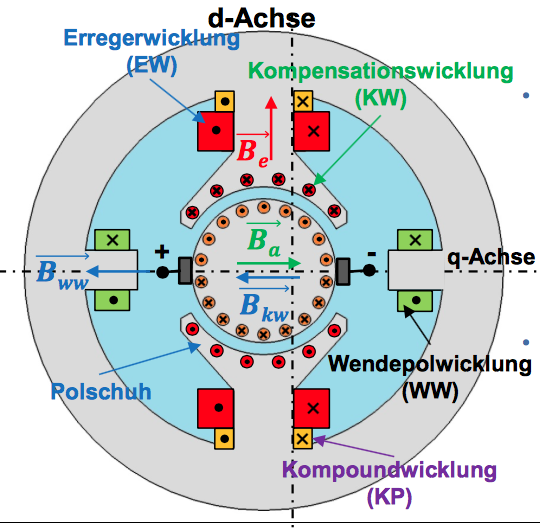
\includegraphics[width = \linewidth]{./Pics/VL45/Wendepolwicklung}
\end{minipage}

\subsection{Arbeitsbereiche und Grenzwerte}

\begin{minipage}{0.4 \linewidth}
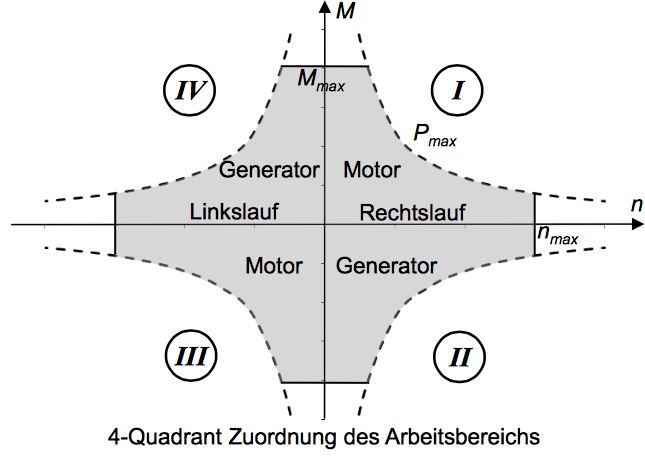
\includegraphics[width = \linewidth]{./Pics/VL45/Arbeitsbereich}
\end{minipage}
\begin{minipage}{0.6 \linewidth}
Im Datenblatt der Maschine werden vom Hersteller die Betriebsgrenzwerte gegeben: \\

$P_{max},M_{max},n_{max},I_{emax}(\Psi_{max}),I_{amax} und U_{amax}$\\

$P = \omega \cdot M = 2 \cdot \pi \cdot n \cdot M$ \\

$M(n) = \frac{P_{max}}{2 \cdot \pi} \cdot \frac{1}{n}$\\
\end{minipage}

\subsection{Nebenschluss und Reihenschluss}
\subsubsection{Nebenschluss}

Die Erreger- und Ankerwicklung werden parallel an die gleiche Spannungsquelle geschaltet. Dei dem Nebenschluss sind die Anker- und Erregerspannung gleich und die Anker- und Erregerstrom unabhängig voneinander.

\begin{minipage}{0.4 \linewidth}
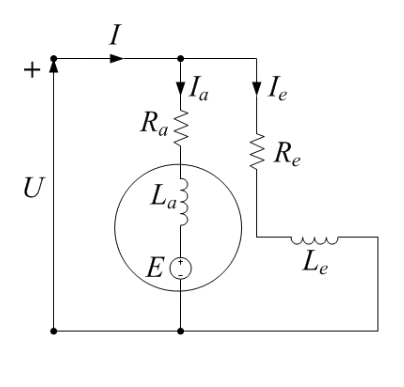
\includegraphics[width = \linewidth]{./Pics/VL45/Nebenschluss}
\end{minipage}
\begin{minipage}{0.6 \linewidth}
Analyse des Drehmoments: \\ 

$M = I_a \cdot \Psi, U = U_a = R_a \cdot I_a + 2 \cdot \pi n \cdot \Psi$ \\

$M = I_a \cdot \Psi = \frac{U \cdot \Psi}{R_a} - \frac{2 \cdot \pi \cdot \Psi^2}{R_a} \cdot n$ \\

Anlaufmoment: \\

$n = 0 \Rightarrow M_a = \frac{U \cdot \Psi}{R_a}$ ($Nm$) \\

Lehrlaufdrehzahl: \\

$M = 0 \Rightarrow n_0 = \frac{U}{2 \cdot \pi \Psi} $ ($\frac{{1}}{s}$)
\end{minipage}

\begin{minipage}{0.4 \linewidth}
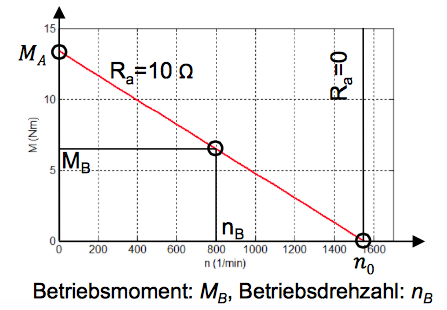
\includegraphics[width = \linewidth]{./Pics/VL45/Nebenschluss2}
\end{minipage}
\begin{minipage}{0.6 \linewidth}
Analyse des Drehmoments: \\

$\frac{M}{M_a} = 1 - \frac{n}{n_0}$\\

$M_a = \frac{U \cdot \Psi}{R_a}$\\

$n_0 = \frac{U}{2 \cdot \pi \cdot \Psi}$
\end{minipage}

\subsubsection{Reihenschluss}
\begin{minipage}{0.3 \linewidth}
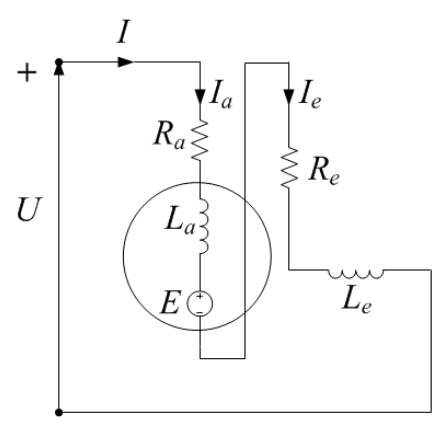
\includegraphics[width = \linewidth]{./Pics/VL45/Reihenschluss}
\end{minipage}
\begin{minipage}{0.7 \linewidth}
Dir Erreger. und Ankerwicklung werden in Serie an die gemeinsame Spannungsquelle geschaltet. Bei dem Reihenschluss sind die Anker- und Erregerstrom gleich und deswegen stark abhängig voneinander. \\

Analyse des Drehmoments: \\

$M = I \cdot \Psi$ \\

$U = (R_a + R_e) \cdot I + 2 \cdot \pi \cdot n \cdot \Psi$ \\

$\Psi = L_e \cdot I$ \\

$M = I \cdot \Psi = L_e (\frac{U}{R_a + R_e + 2 \cdot \pi \cdot n \cdot L_e})^2$ \\

Anlaufmoment: \\

$n = 0 \Rightarrow M_A = \frac{L_e \cdot U^2}{(R_a + R_e)^2}$   $(Nm)$ \\

Bezugsdrehzahl: \\

$n_b = \frac{R_a + R_e}{2 \cdot \pi \cdot L_e}$   $(\frac{1}{s})$
\end{minipage}

\begin{minipage}{0.3 \linewidth}
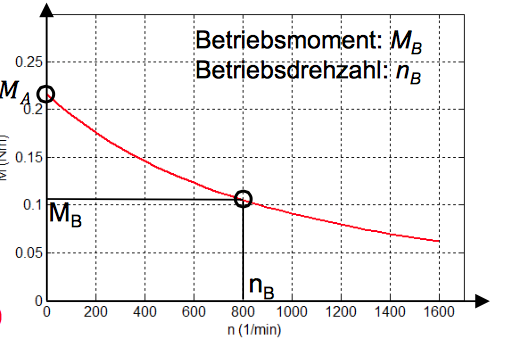
\includegraphics[width = \linewidth]{./Pics/VL45/Reihenschluss2}
\end{minipage}
\begin{minipage}{0.7 \linewidth}
\large{Achtung:} $M \rightarrow 0 \Rightarrow n \rightarrow \inf $\textbf{(Sicherheitsrisiko!)} \\

$\frac{M}{M_A} = \frac{1}{(1 + \frac{n}{n_b})^2} $  \\

$M_A = \frac{L_e \cdot U^2}{(R_a + R_e)^2} $ \\

$n_b = \frac{R_a + R_e}{2 \cdot \pi \cdot L_e}$
\end{minipage}

\subsection{Drehzahlregelung}
\begin{minipage}{0.3 \linewidth}
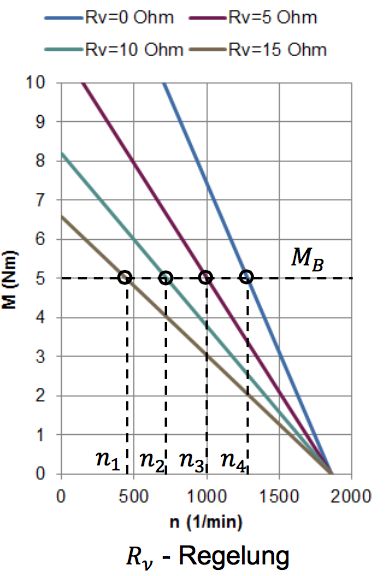
\includegraphics[width = \linewidth]{./Pics/VL45/Drehzahlregelung}
\end{minipage}
\begin{minipage}{0.7 \linewidth}
Die Grundgleichung der Gleichstrommaschine im Nebenschluss: \\

$I_a = \frac{U- 2\cdot\pi \cdot n \cdot \Psi}{R_a}$\\

$M = \frac{U \cdot \Psi}{R_a}- \frac{2\cdot\pi\Psi^2}{R_a}\cdot n$\\

Gemäss den Grundgleichungen sind die Kennlinien $I_a(n)$ und $M(n)$ von $R_a$, $U$ und $\Psi$ stark abhängig. Deswegen wird die Drehzahlregelung durch den zusätzlichen Widerstand $R_v$ im Ankerkreis (verlustreich), durch die Ankerspannung (Verlustarm), oder durch Erregung (Verlustarm) durchgeführt.
\end{minipage}

\begin{minipage}{0.3 \linewidth}
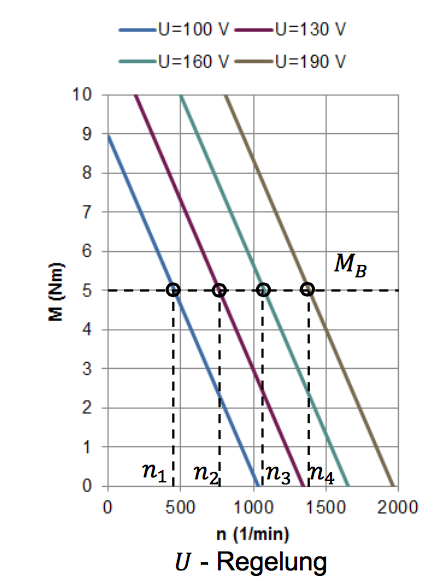
\includegraphics[width = \linewidth]{./Pics/VL45/Drehzahlregelung2}
\end{minipage}
\begin{minipage}{0.3 \linewidth}
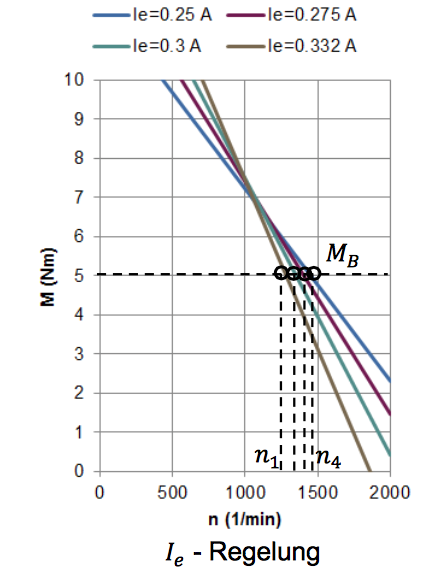
\includegraphics[width = \linewidth]{./Pics/VL45/Drehzahlregelung3}
\end{minipage}

\subsection{Anlauf}
Wegen der Stabilität des Netzwerks muss der Anlaufstrom der Gleichstrommotoren mit einer Leistung über 2 kW begrenzt werden. Ein beispiel der Anlaufstrombegrenzung durch die $R_v$-Regelung sieht so aus: \\

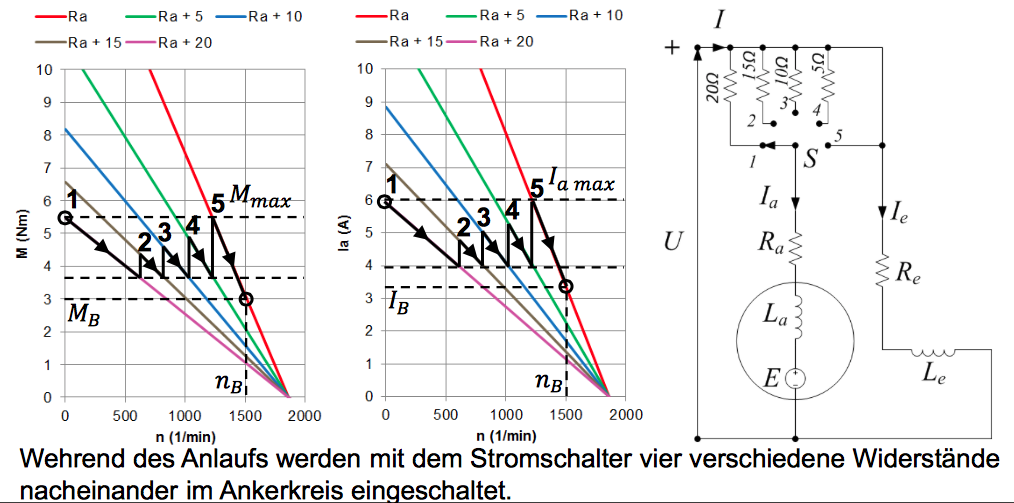
\includegraphics[width = 0.8 \linewidth]{./Pics/VL45/Anlauf}

\subsection{Anwendungsbereiche und Schlussanmerkungen}
\begin{itemize}
\item Die Gleichstrommaschine sind konstruktiv sehr kompliziert und damit auch sehr teuer.
\item Die Gleichstrommaschine mit Fremd-, Neben- und Permanenterregung werden heute nur als Motoren eingesetzt.
\item Die Anwendung in den lokalen Gleichstromnetzen: Fahrzeuge, Schiffe, Batterie-gespeiste Geräte, usw.
\item Spezielle Anwendung wobei stetige Drehzahlregelung erforderlich ist:
\begin{compactitem}
\item Werkzeugmaschine
\item Haspeln
\item Drehrohröfen
\item Papiermaschinen
\item Textilmaschinen,
\item usw.
\end{compactitem}
\item Nebenschluss-GSM: 0.25-3000 kW, 0-3000 $min^{-1}$ (für regelbare Antriebe)
\item Reihenschluss-GSM: 0.5 -1000 kW, 0-10'000 $min^{-1}$ (für Fahrzeugantriebe)
\end{itemize}
\section{Schrittmotor}
\subsection{Reluktanz-Schrittmotor}
\begin{minipage}{0.5 \linewidth}
\subsubsection{Wirkungsprinzip}
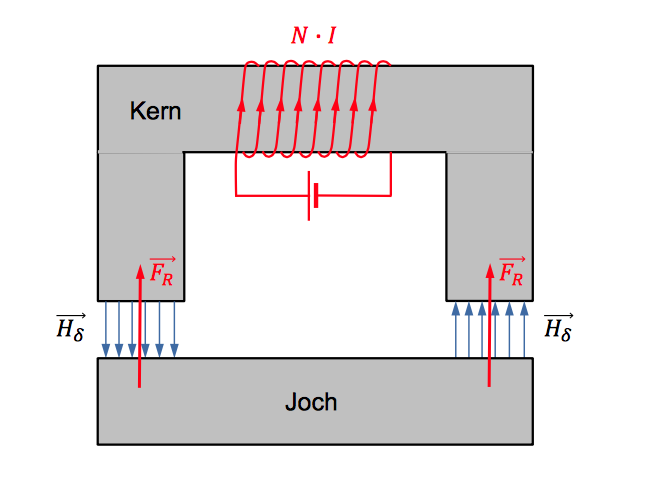
\includegraphics[width = \linewidth]{./Pics/VL67/WirkungRe}
Die magnetische Reluktanzkraft ist immer anziehen, d.h. die Reluktanzkraft versucht die Luftspalte zu verkleinern oder völlig zu eliminieren.
\end{minipage}
\begin{minipage}{0.5 \linewidth}
\subsubsection{Aufbau}
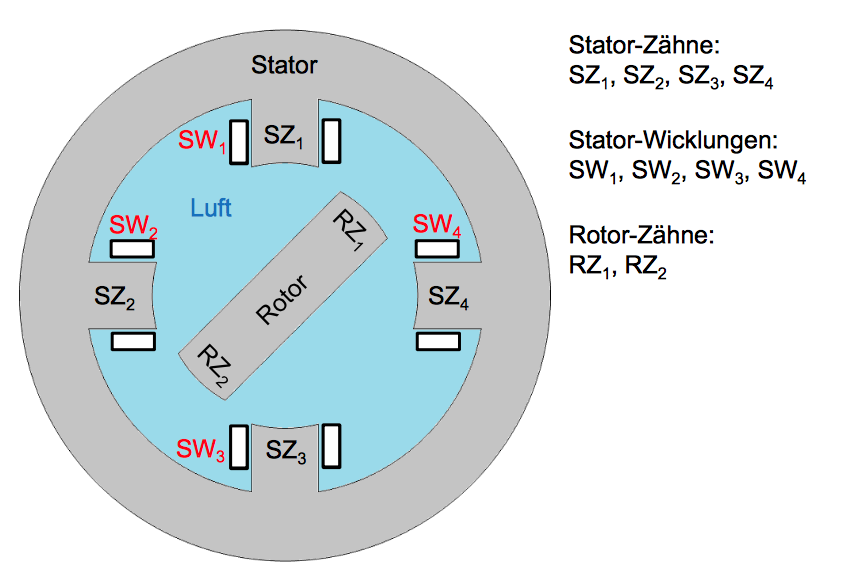
\includegraphics[width = \linewidth]{./Pics/VL67/AufbauRe}
\end{minipage}

\begin{minipage}{0.5 \linewidth}
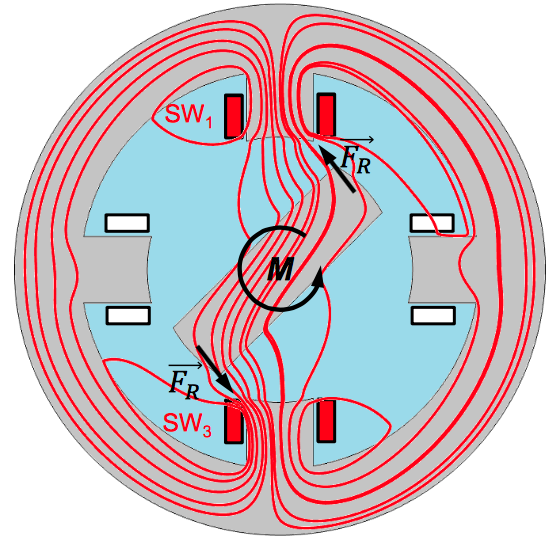
\includegraphics[width = 0.7 \linewidth]{./Pics/VL67/WirkungRe2}
\end{minipage}
\begin{minipage}{0.5 \linewidth}
\begin{itemize}
\item Die Spulen $SW_1$, $SW_3$ sind an die Quelle angeschlossen.
\item Das magnetische Feld der ersten zwei Spulen wird erzeugt.
\item Die Reluktanzkraft wirkt auf den Rotor um die Luftspalte zu verringern.
\item Das mechanische Moment wird erzeugt. 
\end{itemize}
\end{minipage}

\subsection{Permanentmagnet-SM}
\begin{minipage}{0.5 \linewidth}
\subsubsection{Wirkungsprinzip}
\includegraphics[width = \linewidth]{./Pics/VL67/PMSM2}
\end{minipage}
\begin{minipage}{0.5 \linewidth}
\subsubsection{Aufbau}
\includegraphics[width = \linewidth]{./Pics/VL67/PMSM}
\end{minipage}

\subsection{Grundgleichungen}
\begin{minipage}{0.5 \linewidth}
\includegraphics[width = \linewidth]{./Pics/VL67/AufbauRe}
\end{minipage}
\begin{minipage}{0.5 \linewidth}
\subsubsection{Aufbau}
\begin{compactitem}
\item Die Stator-Spulen sind an die Quelle der Steuersignale angeschlossen.
\item Die Steuersignale produzieren das schrittweise Drehen der Motorwelle.
\item Die Stator-Zahnzahl: $Z_S = 4$
\item Die Rotor-Zahnzahl: $Z_R = 2$
\item Der Stator-Winkel: $\alpha_S = \frac{2\cdot \pi}{Z_S} = 90 \deg$
\item Der Rotor-Winkel: $\alpha_R =  \frac{2\cdot \pi}{Z_R} = 180 \deg$
\item Der Vollschritt-Winkel: $\alpha_0 = \alpha_R - \alpha_s = 90 \deg$ 
\item Der Vollschritt-Winkel bezeichnet die Bewegung des Rotors pro Einzelsteuerimpuls.
\item Die Strangzahl: $m = \frac{Z_S}{Z_S - Z_R} = 2$
\item Die Schrittzahl: $N_p = \frac{2\cdot \pi}{\alpha_0} = 4$
\item Die Steuerfrequenz: $f_s = N_p \cdot \frac{n}{60}$ 
\end{compactitem}
\end{minipage}

\subsection{Drehmoment}
\begin{minipage}{0.5 \linewidth}
\includegraphics[width = \linewidth]{./Pics/VL67/Drehmoment}\\
\includegraphics[width = \linewidth]{./Pics/VL67/Drehmoment2} \\

Der magnetische Fluss des Motors: \\

$\Phi_m (\gamma_r,i) = L(\gamma_r(t)) \cdot i(t)$\\

Die Spannung des Statorkreises: 

$u(t)  = R \cdot i(t) + \frac{d\Phi_m}{dt}(t)  = R \cdot i(t) + \frac{d}{dt}(L(\gamma_r(t) \cdot i(t)) \\
 =  R \cdot i(t) + \frac{dL}{d\gamma_r}(\gamma_r) \cdot \frac{d\gamma_r}{dt}i(t) + L(\gamma_r) \cdot \frac{di}{dt}(t)$ \\
 
 Die Leistung des Statorkreises: \\
 
 $p(t) = u(t) \cdot i(t) = R \cdot i^2(t) + \frac{dL}{d\gamma_r} \cdot \omega_r \cdot i^2(t) + L \cdot i(t) \cdot \frac{di}{dt}(t)$\\
 
 Die elektrische Leistung des Stators: 
 
 $p(t) = R \cdot i^2(t) + \frac{dL}{d\gamma_r} \omega_r \cdot i^2(t) + L \cdot i(t) \cdot \frac{di}{dt}(t) \\ 
 = p_{C_u}(t) + \frac{d_{W_m}}{dt}(t) + \frac{1}{2} \cdot \frac{dL}{d \gamma_r}(\gamma_r) \cdot \omega_r \cdot i^2(t)$ \\
 
\end{minipage}
\begin{minipage}{0.5 \linewidth}
Die Induktivität des Statorstrangs (Die Position der d-Achse des Rotor parallel mit dem aktivem Statorzahn): \\

$L_d = 2 \cdot N \frac{\Phi_{md}}{I_1} = 2 \cdot N \frac{B_{\delta d} \cdot A_z}{I_1} = \mu_0 \cdot 2 \cdot N \frac{2 \cdot N \cdot I_1 \cdot A_z}{2 \cdot \delta_d \cdot I_1} = \mu_0 \cdot 2 \cdot N^2 \frac{A_Z}{\delta_d}$ \\

wobei $N$ die Windungszahl des Statorstrangs, $A_Z$ die Zahnfläche und $\delta_d$ die Höhe des Luftspalts (bei der d-Position des Rotors relativ zu dem Statorzahn) ist. \\

Die Induktivität des Statorstrangs hängt offenbar von der Rotorposition ab: \\

\includegraphics[width = \linewidth]{./Pics/VL67/Drehmoment3} \\
\includegraphics[width = \linewidth]{./Pics/VL67/Drehmoment4} \\

Die Zeitableitung der magnetischen Energie: \\

$w_m(t) = \frac{1}{2} L(\gamma_r) \cdot i^2(t) \Rightarrow \frac{d}{dt}(\frac{1}{2}\cdot L(\gamma_r)\cdot i^2(t)) = \\
\frac{1}{2} \cdot \frac{dL}{d\gamma_r}(\gamma_r) \cdot \omega_r \cdot i^2(t) + L \cdot i(t) \cdot \frac{di}{dt}(t)$
\end{minipage}

\begin{minipage}{0.5 \linewidth}
\includegraphics[width = \linewidth]{./Pics/VL67/Drehmoment5}
\end{minipage}
\begin{minipage}{0.5 \linewidth}
Die Rotorleistung: \\

$P_\delta (t) = \frac{1}{2} \cdot \frac{dL}{d\gamma_r}\cdot(\gamma_R) \cdot \omega_r \cdot i^2(t)$ \\

Das Motormoment: 

$m_M(t) = \frac{p_\gamma}{\omega_r}(t) = \frac{1}{2} \cdot \frac{dL}{d\gamma_r}(\gamma_r) \cdot i^2(t)$\\

Das Betriebsverhalten des Motors beschreibt die folgende Gleichung: 

$J_g \frac{d\omega_r}{dt} = M_M - M_L $\\

wobei $J_g$ das gesamte motorbezogene Trägheitsmoment des System, $M_M$ das Drehmoment des Motors und $M_L$ das Widerstandsmoment der Last ist.\\
\end{minipage}

\begin{minipage}{0.5 \linewidth}
\includegraphics[width = \linewidth]{./Pics/VL67/Betriebsverhalten}
\end{minipage}
\begin{minipage}{0.5 \linewidth}
Die Differenzialgleichung der Rotorbewegung (mit der linearen Annäherung der Winkelbeschleunigung): \\

$J_g \frac{\omega_s-\omega_1}{T_s} = M_M - M_L$ \\

wobei $\omega_s = 2 \cdot \pi \frac{n_s}{60} = 2 \cdot \pi \frac{f_s}{N_p} = a_0 f_s$ die Kreisgeschwindigkeit des Statorfelds, $\omega_1$ die geometrische Kreisgeschwindigkeit des Rotors in dem Moment des Impulseinschaltens ($\omega_1 = 0$ bedeutet der Rotor im Stillstand), $f_s = \frac{1}{T_s}$ die Frequenz der Statorimpulse ist. \\

Die Gleichung beschreibt die Beschleunigung des Rotors während einem Statorimpuls. Der Rotor muss von der Geschwindigkeit $\omega_1$ auf die Geschwindigkeit $\omega_s$ beschleunigen. Sonst wird der Rotor ausser Tritt geraten. \\

Das Lastmoment $M_L$ als eine Funktion der Schaltfrequenz und Anfangsgeschwindigkeit: \\

$M_L(f_s,\omega_1) = M_M-J_g\frac{\omega_s}{T_s} + J_g\frac{\omega_1}{T_s} \\
= M_M-J_g\omega_s f_s + J_g \omega_1 f_s\\
= M_M - J_g \alpha_0 f_s^2 + J_g \omega_1 f_s$\\
\end{minipage}

\begin{minipage}{0.5 \linewidth}
\subsection{Anwendungsbereich und Schlussanmerkung}
\begin{itemize}
\item Die Schrittmotoren sind für die Anwendung mit Bewegungsführung geeignet.
\item Die Schrittmotoren sind sehr kostengünstig.
\item Die Schrittmotoren sind praktisch nicht überlastbar.
\item Die wichtigsten Anwendungen:
\begin{itemize}
\item Arbeitsmaschine
\item Datenausgabegeräte (Plotter, Drucker, usw.)
\end{itemize}
\item Die Schrittmotoren geben einen Drehmoment von bis zu 5 Nm ab.
\item Die Schrittmotoren werden im unteren Leistungsbereich eingesetzt. 
\end{itemize}
\end{minipage}
\begin{minipage}{0.5 \linewidth}
\subsection{Drehzahlregelung und Anlauf}
\includegraphics[width = \linewidth]{./Pics/VL67/Drehzahl}
\end{minipage}



\end{document}
